\nocite{anleitungV351}
\section{Zielsetzung}
\label{sec:Zielsetzung}
Das Ziel dieses Versuchs ist aus Fourierkomponenten eine Funktion zu synthetisieren sowie verschiedene Funktionen 
in einzelne Fourierkomponente zu zerlegen. 
\section{Theorie}
\label{sec:Theorie}
Wenn sich eine Funktion nach einer festen Zeit oder einer festen Distanz wiederholt, heißt diese periodisch. Für eine
zeitlich periodische Funktion mit Periodendauer $T$ gilt
\begin{equation}
    f(t+T) = f(t)\,.
    \label{eqn:zeitlichPeriodisch}
\end{equation}
Eine räumlich periodische Funktion erfüllt die Beziehung 
\begin{equation}
    f(x+D) = f(x)\,.
    \label{eqn:räumlichPeriodisch}
\end{equation}
Die beiden wichtigsten periodischen Funktionen sind die Sinus- und Cosinusfunktionen. Im Allgemeinen lassen sich die beiden
Funktionen mit 
\begin{align}
    f(t)& = a\sin\left(\frac{2\pi}{T}\cdot t\right)\quad\text{bzw.} \label{eqn:allgSinus}\\
    f(t)& = b\cos\left(\frac{2\pi}{T}\cdot t\right) \label{eqn:allgCosinus}
\end{align}
beschreiben. Hierbei ist $a$ bzw. $b$ die jeweilige Amplitude und $T$ die Periodendauer. Mithilfe dieser beiden Funktionen 
lassen sich viele periodische Vorgänge der Natur beschreiben. Dies folgt aus dem Fourierschen Theorem
\begin{equation}
    \frac{1}{2}a_0 + \sum_{n=1}^{\infty}\left(a_n\cos\left(\frac{2\pi n}{T}\cdot t\right)+b_n\sin\left(\frac{2\pi n}{T}\cdot t\right)\right)\,.
    \label{eqn:FourierTheorem}
\end{equation}
Wenn diese Reihe gleichmäßig konvergiert, dann stellt die Fourier-Entwicklung in Gleichung (\ref{eqn:FourierTheorem}) eine periodische 
Funktion $f(t)$ dar. Die Funktion ist gleichmäßig konvergent, wenn diese an jeder Stelle stetig ist. Falls eine Funktion an einer Stelle $t_0$
nicht stetig ist, lässt sich diese Funktion bei $t_0$ nicht mit der Fourier-Reihe annähern. Stattdessen tritt an der Stelle $t_0$ eine endliche Abweichung
auf. Diese Beobachtung wird Gibbsches Phänomen gannant. Die Koeffizienten $a_n$ und $b_n$ lassen sich für $n \in \mathbb{N}$ wie folgt berechnen
\begin{align}
    a_n &= \frac{2}{T} \int_{0}^{T}f(t)\cos \left( \frac{2\pi n}{T}\cdot t\right)\text{d}t\quad \text{bzw.} \label{eqn:a_n}\\
    b_n &= \frac{2}{T} \int_{0}^{T}f(t)\sin \left( \frac{2\pi n}{T}\cdot t\right)\text{d}t\,.\label{eqn:b_n}
\end{align}
Die Bestimmung dieser Koeffizienten bzw. Amplituden wird Fourier-Analyse genannt. Falls $f(t)$ eine gerade Funktion ist, also $f(t)=f(-t)$, dann 
gilt $b_n = 0\,\,\forall n$. Für eine ungerade Funktion $f(t)$, also wenn $f(t) = -f(-t)$ gilt, dann gilt $a_n= 0\,\,\forall n$.
Die Grundfrequenz der Schwingungen wird durch
\begin{equation}
    \nu_1=\frac{1}{T}
    \label{eqn:Grundfrequenz}
\end{equation}
beschrieben. Die restlichen Frequenzen des periodischen Vorgangs der Fourier-Entwicklung sind ganzzahlige Vielfache von
der Grundfrequenz $\nu_1$. Diese Frequenzen heißen harmonische Oberschwingungen und treten nur in den Phasen $0,\,\, \frac{\pi}{2}$ und $\frac{3}{2}\pi$
auf. Werden die Amplituden der Oberschwingungen als Funktion der Frequenz aufgetragen, so ergibt sich das Spektrum der Schwingung. Bei periodischen
Funktionen ensteht ein Linienspektrum wie in Abbildung (\ref{fig:Linienspektrum}) zu erkennen. Dahingegen weisen nicht-periodische Vorgänge ein
kontinuierliches Spektrum auf.
\begin{figure}[H]
    \centering
    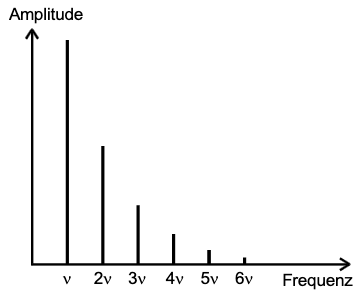
\includegraphics[width=0.50\textwidth]{Linienspektrum.png}
    \caption{Beispiel eines Linienspektrums einer periodischen Funktion. [Q\cite{anleitungV351}]}
    \label{fig:Linienspektrum}
\end{figure}
Mithilfe der Fourier-Transformation
\begin{equation}
    g(\nu)= \int_{-\infty}^{\infty}f(t)\exp\left(i \nu t\right) \text{d}t
    \label{eqn:FourierTransformation}
\end{equation}
lässt sich das gesamte Frequenzspektrum einer zeitabhängigen Funktion bestimmen. Diese gilt sowohl für periodische als auch für 
nicht-periodische Funktionen. Die umgekehrte Fourier-Transformation lautet
\begin{equation}
    f(t)=\frac{1}{2\pi}\int_{\infty}^{\infty}g(\nu)\exp\left(-i\nu t\right)\text{d}\nu\,.
    \label{eqn:reverseFourierTransformation}
\end{equation}
Im Allgemeinen ist zu beachten, dass oftmals eine Integration über einen unendlich langen Zeitraum nicht möglich ist, weswegen die Integration auf einen endlichen
Zeitraum beschränkt wird. Daher ist die Periodizität von der Funktion $f(t)$ nicht mehr erfüllt.
\section{Vorbereitungsaufgabe}
\label{sec:Vorbereitungsaufgabe}
